\renewcommand{\NomeBloco}{\textit{Comparador}}
\renewcommand{\NomeBlocoNoIt}{Comparador}
\renewcommand{\NomePTab}{tab_\NomeBloco}
\renewcommand{\NomeSTab}{tab_\NomeBlocoNoIt2}
\renewcommand{\NomePFig}{fig_\NomeBlocoNoIt}
\renewcommand{\NomeSFig}{fig_\NomeBlocoNoIt2}
\renewcommand{\NomeTTab}{tab_\NomeBlocoNoIt3}

\section{Comparador}

O bloco \NomeBloco{} tem a função de comparar dois sinais anal\'ogicos advindos nas entradas '+' (\textit{Vp}) e '-' (\textit{Vn}), e retornar \textit{VDD} caso Vp seja maior do que Vn, e \textit{GND} caso Vp seja menor ou igual a Vn. O bloco apresenta as definições de sinais de entrada e sa\'ida referidos na \autoref{\NomeSTab}.

\begin{table}[!h]
\caption{Sinais do bloco \NomeBloco}
\label{\NomeSTab}
\centering
\begin{tabular}{ccl}

    \toprule
    Sinal & Tipo    & Descrição        \\
    \midrule \midrule
    Vp (+) & Entrada & Entrada positiva do Comparador\\
    \midrule
    Vn (-) & Entrada & Entrada negativa do Comparador\\
    \midrule
    Ibias & Entrada & Corrente de polarização do Comparador\\
    \midrule
    Vo & sa\'ida & Sa\'ida do Comparador\\
    \bottomrule
\end{tabular}
\legend{Fonte: Produzido pelo autor}
\end{table}

O circuito projetado para o bloco \'e demonstrado na \autoref{\NomePFig}.

\begin{figure}[!h]
 \centering
    \centering
    \caption{Circuito CMOS projetado para o bloco \NomeBloco} 
    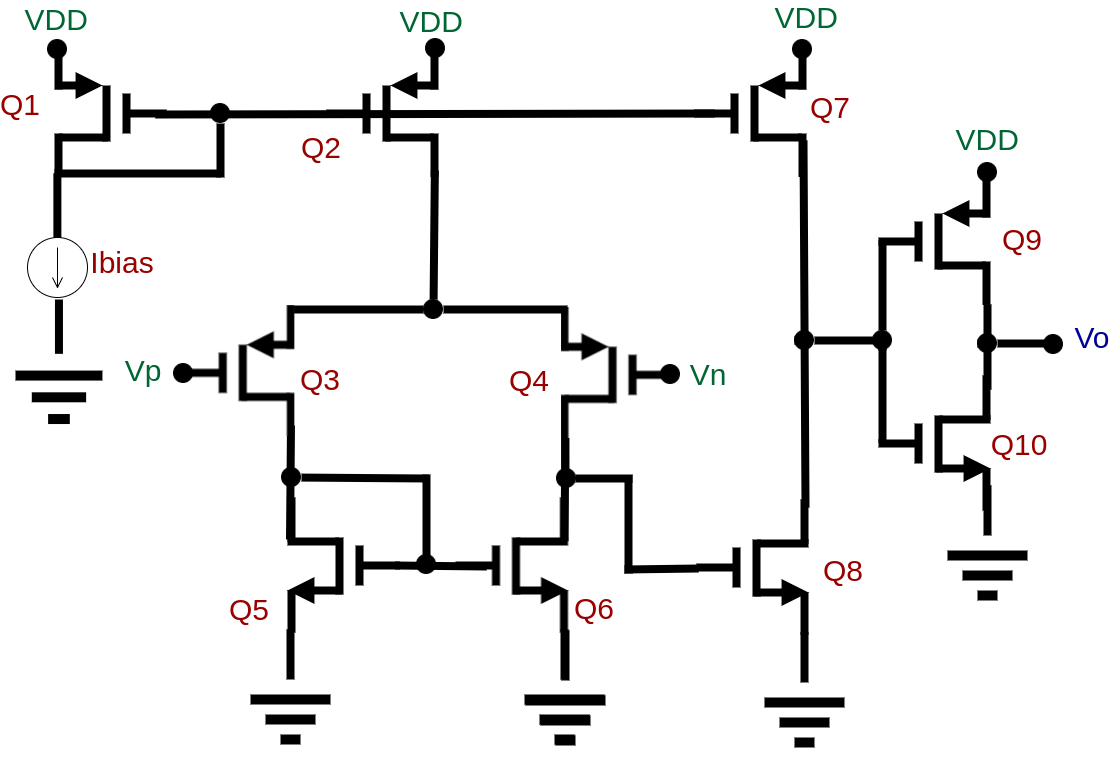
\includegraphics[scale=0.3]{Circuitos/Comparator.png}
    \legend{Fonte: Produzido pelo autor}
    \label{\NomePFig}
\end{figure}

\begin{figure}[!h]
 \centering
    \centering
    \caption{\label{\NomeSFig}Representação em bloco do \NomeBloco}
    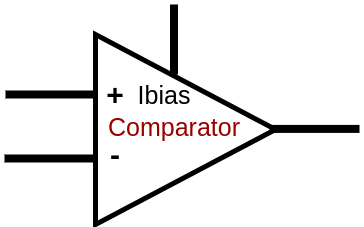
\includegraphics[scale=0.3]{Circuitos/Comparator_block.png}
    \legend{Fonte: Produzido pelo autor}
\end{figure}

Os transistores utilizados no bloco \NomeBloco{} apresentam os par\^ametros mostrados na \autoref{\NomeTTab}.

\begin{table}[!h]
\caption{Transistores do Bloco \NomeBloco}
\label{\NomeTTab}
\centering
\begin{tabular}{ccccc}
\toprule
Transistor & W ($\mu$m)  & L ($\mu$m)           & M (n° dispositivos) & S (n° dispositivos)\\
\midrule \midrule
Q1 & 10 & 1 & 1 & 1\\
\midrule
Q2$^1$ & 10 & 1 & 6 & 6\\
\midrule
Q3 & 4 & 1 & 2 & 2\\
\midrule
Q4 & 4 & 1 & 2 & 2\\
\midrule
Q5 & 2 & 1 & 2 & 2\\
\midrule
Q6 & 2 & 1 & 2 & 2\\
\midrule
Q7$^1$ & 10 & 1 & 8 & 8\\
\midrule
Q8 & 2 & 1 & 4 & 4\\
\midrule
Q9 & 3 & 0.18 & 1 & 1\\
\midrule
Q10 & 1.5 & 0.18 & 1 & 1\\

\bottomrule
\end{tabular}
\legend{Fonte: Produzido pelo autor}
\legend{$^1$Calculado de forma a produzir uma corrente de 9 $\mu$A}
\end{table}
 
O \NomeBloco{} \'e desenvolvido com dois est\'agios de amplificação. O primeiro est\'agio, composto pelos transistores Q3, Q4, Q5, Q6 t\^em a função de realizar a diferença entra as entradas \textit{Vp} e \textit{Vn} e multiplicar por um pequeno ganho. Os transistores Q3 e Q4 são respons\'aveis por receber as entradas, enquanto os transistores Q5 e Q6 funcionam como transistores de Carga Ativa. O Q2 funciona como uma fonte de corrente.

O segundo est\'agio \'e um est\'agio de ganho, do qual o transistor Q2 fornece um ganho para a saía do est\'agio anterior e o transistor Q7 funciona como uma fonte de corrente para o est\'agio.

Diodos quadrados \textit{D1} e \textit{D2} de proteção são inclu\'idos nos terminais \textit{Vp} e \textit{Vn do circuito}, com \^anodo ligado ao terra e catodo ligado ao seu respectivo terminal. Os diodos apresentam os seguintes par\^ametros apresentados na \autoref{diodosComp}.

\begin{table}[!h]
\caption{Diodos do Bloco \NomeBloco}
\label{diodosComp}
\centering
\begin{tabular}{cccc}
\toprule
Diodo & W ($\mu$m)  & L ($\mu$m)           & \'Area ($\mu$m²)\\
\midrule \midrule
D1 e D2 & 1 & 1 & 1 \\

\bottomrule
\end{tabular}
\legend{Fonte: Produzido pelo autor}
\end{table}
